\label{boundary-conditions}
\subsection*{Introduction}

\D is designed to accommodate a number of different periodic
boundary conditions\index{boundary conditions}, which are defined
by the shape and size of the simulation cell.  Briefly, these are
as follows (which also indicates the IMCON flag defining the
simulation cell type in the CONFIG file - see \ref{config-file}):
\begin{tabbing}
XX\=XX\=XXXXXXXXXXXXXXXXXXXXXX\=XXXXX\=\kill
 \> 1. \> None e.g. isolated polymer in space                  \> (${\tt imcon}~=~0$) \\
 \> 2. \> Cubic periodic boundaries\index{boundary conditions} \> (${\tt imcon}~=~1$) \\
 \> 3. \> Orthorhombic periodic boundaries                     \> (${\tt imcon}~=~2$) \\
 \> 4. \> Parallelepiped periodic boundaries                   \> (${\tt imcon}~=~3$) \\
 \> 5. \> Slab (X,Y periodic; Z non-periodic)                  \> (${\tt imcon}~=~6$)
\end{tabbing}
We shall now look at each of these in more detail.  Note that in
all cases the cell vectors and the positions of the atoms in the
cell are to be specified in Angstroms (\AA).

\subsubsection*{No periodic boundary (${\tt imcon}~=~0$)}

Simulations requiring no periodic boundaries are best suited to
{\em in vacuuo} simulations, such as the conformational study of
an isolated polymer molecule.  This boundary condition is not
recommended for studies in a solvent, since evaporation is likely
to be a problem.

Note this boundary condition have to be used with caution.  \D is
not naturally suited to carry out efficient calculations on
systems with great fluctuation of the local density in space, as
is the case for clusters in vacuum.  The parallelisation and
domain decomposition is therefore limited to eight domains
(maximum of two in each direction in space).

This boundary condition should not used with the SPM Ewald
summation method.


\subsubsection*{Cubic periodic boundaries (${\tt imcon}~=~1$)}

\begin{figure}[htbp]
\begin{center}
\vskip 1ex
\centerline{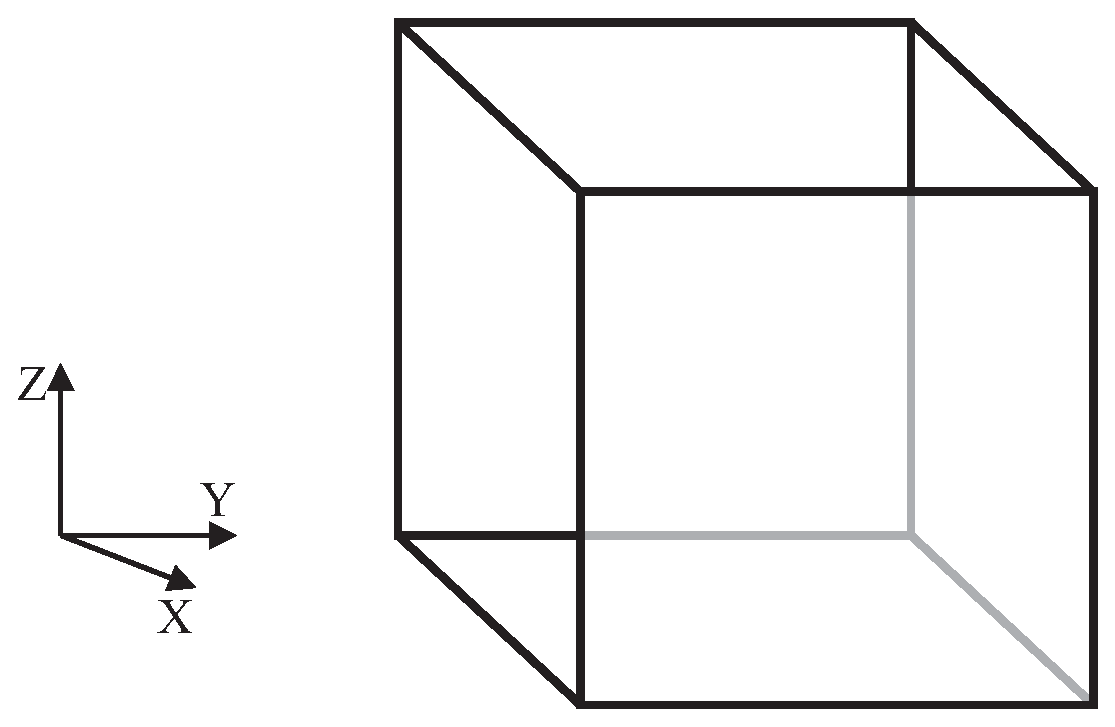
\includegraphics[height=5.0cm]{cube.eps}}
\caption{The cubic MD cell}
%\vskip 1ex
\end{center}
\end{figure}

The cubic MD cell is perhaps the most commonly used in simulation
and has the advantage of great simplicity.  In \D the cell is
defined with the principle axes passing through the centres of the
faces.  Thus for a cube with sidelength D, the cell vectors
appearing in the CONFIG file should be: (D,0,0); (0,D,0); (0,0,D).
Note the origin of the atomic coordinates is the centre of the
cell.

\subsubsection*{Orthorhombic periodic boundaries (${\tt imcon}~=~2$)}

\begin{figure}[htbp]
\begin{center}
\vskip 1ex
\centerline{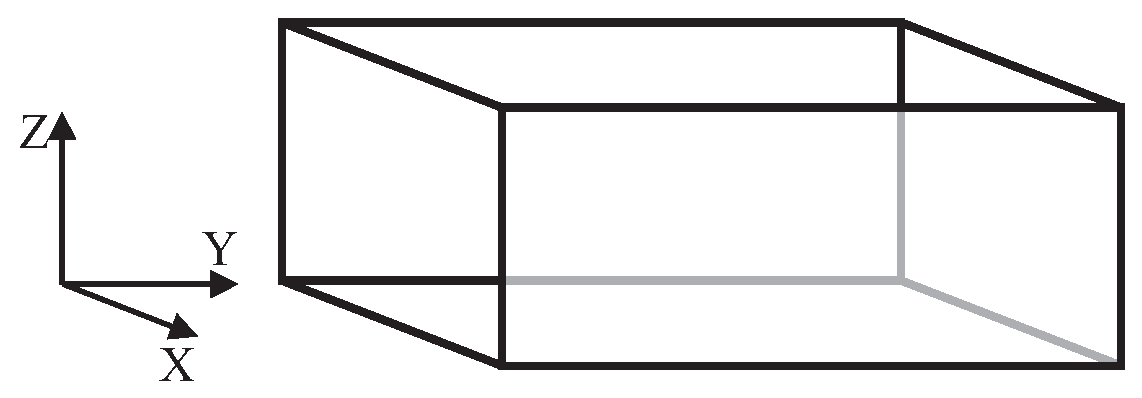
\includegraphics[height=2.7cm]{ortho.eps}}
\caption{The orthorhomic MD cell}
%\vskip 1ex
\end{center}
\end{figure}

The orthorhombic cell is also a common periodic boundary, which
closely resembles the cubic cell in use.  In \D the cell is
defined with principle axes passing through the centres of the
faces.  For an orthorhombic cell with sidelengths D (in
X-direction), E (in Y-direction) and F (in Z-direction), the cell
vectors appearing in the CONFIG file should be: (D,0,0); (0,E,0);
(0,0,F).  Note the origin of the atomic coordinates is the centre
of the cell.

\subsubsection*{Parallelepiped periodic boundaries (${\tt imcon}~=~3$)}

\begin{figure}[htbp]
\begin{center}
\vskip 1ex
\centerline{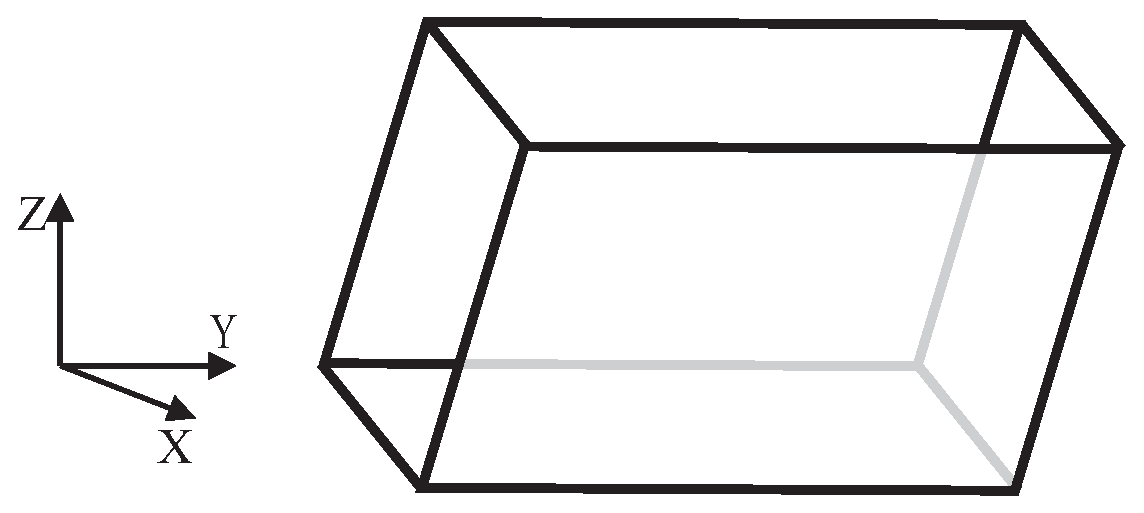
\includegraphics[height=3.5cm]{triclinic.eps}}
\caption{The parallelepiped MD cell}
%\vskip 1ex
\end{center}
\end{figure}
The parallelepiped (e.g. monoclinic or triclinic) cell is
generally used in simulations of crystalline materials, where its
shape and dimension is commensurate with the unit cell of the
crystal.  Thus for a unit cell specified by three principal
vectors $\vek{a}$, $\vek{b}$, $\vek{c}$, the MD cell is defined in
the \D CONFIG file by the vectors (L$a_{1}$,L$a_{2}$,L$a_{3}$),
(M$b_{1}$,M$b_{2}$,M$b_{3}$), (N$c_{1}$,N$c_{2}$,N$c_{3}$), in
which L,M,N are integers, reflecting the multiplication of the
unit cell in each principal direction.  Note that the atomic
coordinate origin is the centre of the MD cell.

\subsubsection*{Slab boundary conditions (${\tt imcon}~=~6$)}

Slab boundaries are periodic in the X- and Y-directions, but not
in the Z-direction.  They are particularly useful for simulating
surfaces. The periodic cell in the XY plane can be any
parallelogram.  The origin of the X,Y atomic coordinates lies on
an axis perpendicular to the centre of the parallelogram.  The
origin of the Z coordinate is where the user specifies it.
However, it is recommended that it is in the middle of the slab.
Domain decomposition division across Z axis is limited to $2$.

If the XY parallelogram is defined by vectors $\vek{A}$ and
$\vek{B}$, the vectors required in the CONFIG file are:
(A$_{1}$,A$_{2}$,0), (B$_{1}$,B$_{2}$,0), (0,0,D), where D is any
real number (including zero).  If D is nonzero, it will be used by
DL\_POLY to help determine a `working volume' for the system. This
is needed to help calculate RDFs etc.  (The working value of D is
in fact taken as one of: 3$\times$cutoff; or 2$\times$max~abs(Z
coordinate)+cutoff; or the user specified D, whichever is the
larger.)

The surface in a system with charges can also be modelled with \D
if periodicity is allowed in the Z-direction. In this case slabs
of ions well-separated by vacuum zones in the Z-direction can be
handled with {\tt imcon}~= 1, 2 or 3.
